\paragraph{Branch Predictor}

\begin{figure}[H]
    \centering
    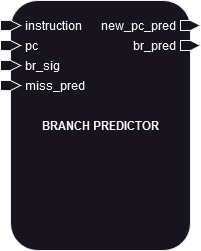
\includegraphics[width=0.35\textwidth]{design/pipelined/fetch/images/br_predictor.png}
    \caption{Diagram of the Branch Predictor}
    \label{fig:br_predictor}
\end{figure}

The branch predictor as its name suggests is responsible for predicting if the branch will be taken or not. The algorithm that 
is being used is the two-level adaptive branch predictor~\cite{two_level_adaptive}, which I will not describe in detail but reuse the idea of a 
2-bit saturating counter but apply a bit of the notion of locality and pattern recognition. Of course, the algorithm
could be improved or replaced by any other algorithm and it is up to the user to do it if he wants to.
It works at the beginning by doing a simple matching on the current instruction to see if it is a branch instruction.
If that's the case we look if it is a conditional branch or not, if it is not we simply predict that the branch will be taken for 
the JAL instruction, but the JALR one will be always predicted as not taken for data dependency reasons. If it is a conditional branch
we simply use the algorithm described above to predict if the branch will be taken or not. The algorithm updates the prediction depending 
on the actual result of the branch that is represented by the $miss\_pred$ signal. If the prediction is taken, we compute the next PC \\

Signals:
\begin{enumerate}[label={\textbullet}]
    \item Input: $instruction$, This signal is representing the current instruction that is being fetched.
    \item Input: $pc$, This signal is representing the current PC.
    \item Input: $br\_sig$ This signal is representing the state of the current instruction in the EX stage. It is used to know if the instruction is a branch or not.
    such that it updates only the algorithm when it is a branch instruction.
    \item Input: $miss\_pred$, This signal is representing the state of the prediction made by the branch predictor in the EX stage.
    \item Output: $new\_pc\_pred$, This signal is representing the next PC that will be used if the prediction is taken.
    \item Output: $br\_pred$, This signal is indicating if the branch is predicted as taken or not.
\end{enumerate}
